\documentclass[tikz,border=3.14mm]{standalone}
%%%%%%%%%%%%%%%%%
%Donut Chart
%%%%%%%%%%%%%%%%%%%%
\def\innerradius{0.7cm}
\def\outerradius{1.9cm}
\pgfmathsetlengthmacro{\centerradius}{(\outerradius + \innerradius)/2}
\pgfmathsetlengthmacro{\donutcenter}{\innerradius/2}
 % The Macro from https://tex.stackexchange.com/q/301199/121799
\newcommand{\donutchart}[1]{
   % Calculate total
   \pgfmathsetmacro{\totalnum}{0}
   \foreach \value/\colour/\name in {#1} {
     \pgfmathparse{\value+\totalnum}
     \global\let\totalnum=\pgfmathresult
   }


  \pgfmathsetmacro{\wheelwidth}{\outerradius-\innerradius}
  \pgfmathsetmacro{\midradius}{(\outerradius+\innerradius)/2}

  \begin{scope}[rotate=90]

    \pgfmathsetmacro{\cumnum}{0}
    \foreach \value/\colour/\name in {#1} {
        \pgfmathsetmacro{\newcumnum}{\cumnum + \value/\totalnum*360}

        \pgfmathsetmacro{\midangle}{-(\cumnum+\newcumnum)/2}

        \filldraw[draw=white,fill=\colour] (-\cumnum:\outerradius) arc (-\cumnum:-(\newcumnum):\outerradius) --
        (-\newcumnum:\innerradius) arc (-\newcumnum:-(\cumnum):\innerradius) -- cycle;

        \fill[darkgray!15] circle (\innerradius);

        \draw node [text=white, font=\sffamily,align=center] at (\midangle:{\innerradius+\wheelwidth/2}) {\name};

        \node[scale=1.0, color=darkgray, font=\sffamily,align=center](\innerradius)
        {Root};

        \global\let\cumnum=\newcumnum
    }

  \end{scope}

  }

\begin{document}

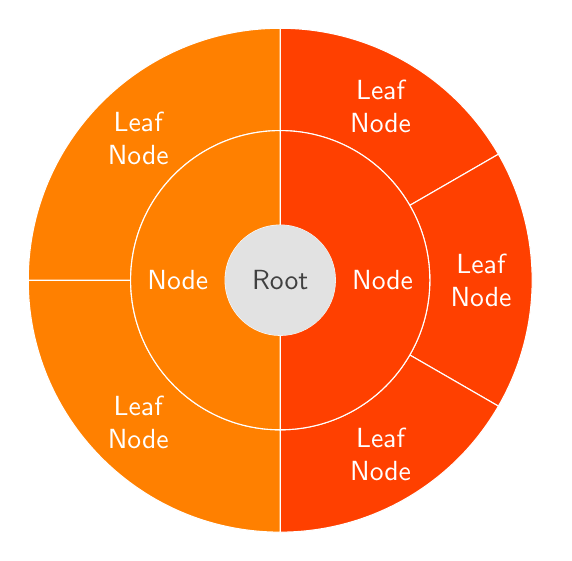
\begin{tikzpicture}[font=\sffamily] 
\def\innerradius{1.9cm}
\def\outerradius{3.2cm}
\pgfmathsetlengthmacro{\centerradius}{(\outerradius + \innerradius)/2}
\pgfmathsetlengthmacro{\donutcenter}{\innerradius/2}

\donutchart{2/orange!50!red/Leaf\\ Node,2/orange!50!red/Leaf\\ Node,
2/orange!50!red/Leaf\\ Node,3/orange/Leaf\\ Node,3/orange/Leaf\\ Node}

\def\innerradius{0.7cm}
\def\outerradius{1.9cm}
\pgfmathsetlengthmacro{\centerradius}{(\outerradius + \innerradius)/2}
\pgfmathsetlengthmacro{\donutcenter}{\innerradius/2}

\donutchart{1/orange!50!red/Node,1/orange/Node}
\end{tikzpicture}
\end{document}
